\documentclass [titlepage,12pt,letter] {article}
\pagestyle{myheadings}


\usepackage{graphicx} 
\usepackage{epsfig}
\usepackage{subfigure}
\usepackage{fancyhdr}
\usepackage{url} 
\usepackage{amsmath}
\usepackage{algorithm} 
\usepackage{algorithmic}
\usepackage{enumerate}
\pagestyle{fancy}



\fancyhead{}
\fancyfoot{}
			
\lhead{CSC349A Lecture Notes}
\rhead{Little, Rich}


\setcounter{page}{1}
\cfoot{\thepage}




\begin{document} 


These are the lecture notes for CSC349A Numerical Analysis taught by
Rich Little. They roughly correspond to
the material covered in each lecture in the classroom but the actual
classroom presentation might deviate significantly from them depending
on the flow of the course delivery. They are provided as a reference to
the instructor as well as supporting material for students who miss
the lectures. They are simply notes to support the lecture so the text
is not detailed and they are not thoroughly checked. Use at your own
risk. They are complimentary to the handouts. Many thanks to all the
guidance and materials I received from Dale Olesky who has taught this
course for many years and George Tzanetakis. 




\section{Spline Interpolation} 

An alternative to polynomial interpolation use ``piecewise'' polynomials. 
\\
Given $x_0, x_1, \dots, x_n$ and $f(x_0), f(x_1), \dots, f(x_n)$ 
construct a different interpolating polynomial on each subinterval: 

\[
[x_0, x_1], [x_1, x_2], \dots, [x_{n-1}, x_n] 
\]
\noindent 
For example piecewise linear interpolation: construct a linear polynomial on each subinterval $[x_i, x_{i+1}]$. 
\\

\begin{figure} 
  \centering
  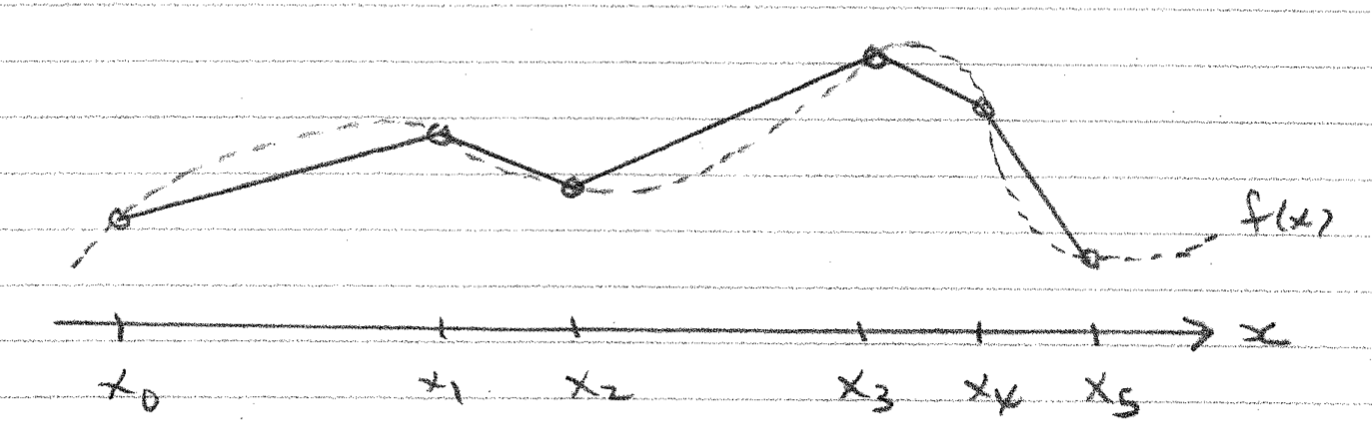
\includegraphics[scale=0.6]{linear_splines}
  \caption{Example of linear spline}
  \label{fig:linear}
\end{figure}



Disadvantage of piecewise linear polynomials: 
not differentiable (at points $x_i$, the knots). 

Differentiability can be obtained by using quadratic (instead of linear) 
polynomials on each $[x_i, x_{i+1}]$. 


\begin{figure} 
  \centering
  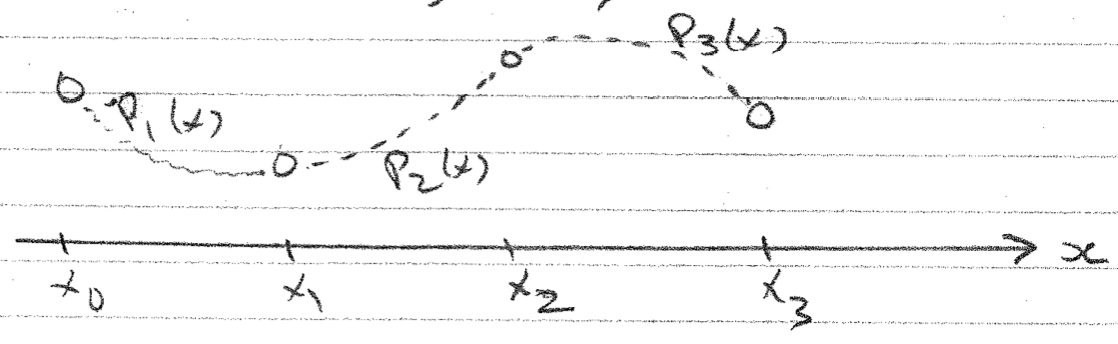
\includegraphics[scale=0.7]{quadratic_splines}
  \caption{Example of quadratic spline}
  \label{fig:linear}
\end{figure}



\begin{itemize} 
\item Each $P_i(x)$ is a quadratic (and is not uniquely determined) 
\item The piecewise polynomial can be made differentiable on $[x_0, x_n]$ 
\item If differentiable, this is an example of a spline function 
\end{itemize}  
\medskip 
\noindent 
{\bf Definition} 
$S(x)$ is a spline function on $[x_0, x_n]$ if for some $q \geq 1$ 
\begin{enumerate} 
\item $S(x)$ is a polynomial of degree $q$ on each subinterval $[x_i, x_{i+1}]$ 
\item $S(x)$ and its first $q-1$ derivatives are continuous on $x_0, x_n$ 
\end{enumerate} 

\begin{itemize} 
\item Linear spline, $q=1$
\item Quadratic spline, $q=2$
\item Cubic spline, $q=3$
\end{itemize} 

\begin{figure} 
  \centering
  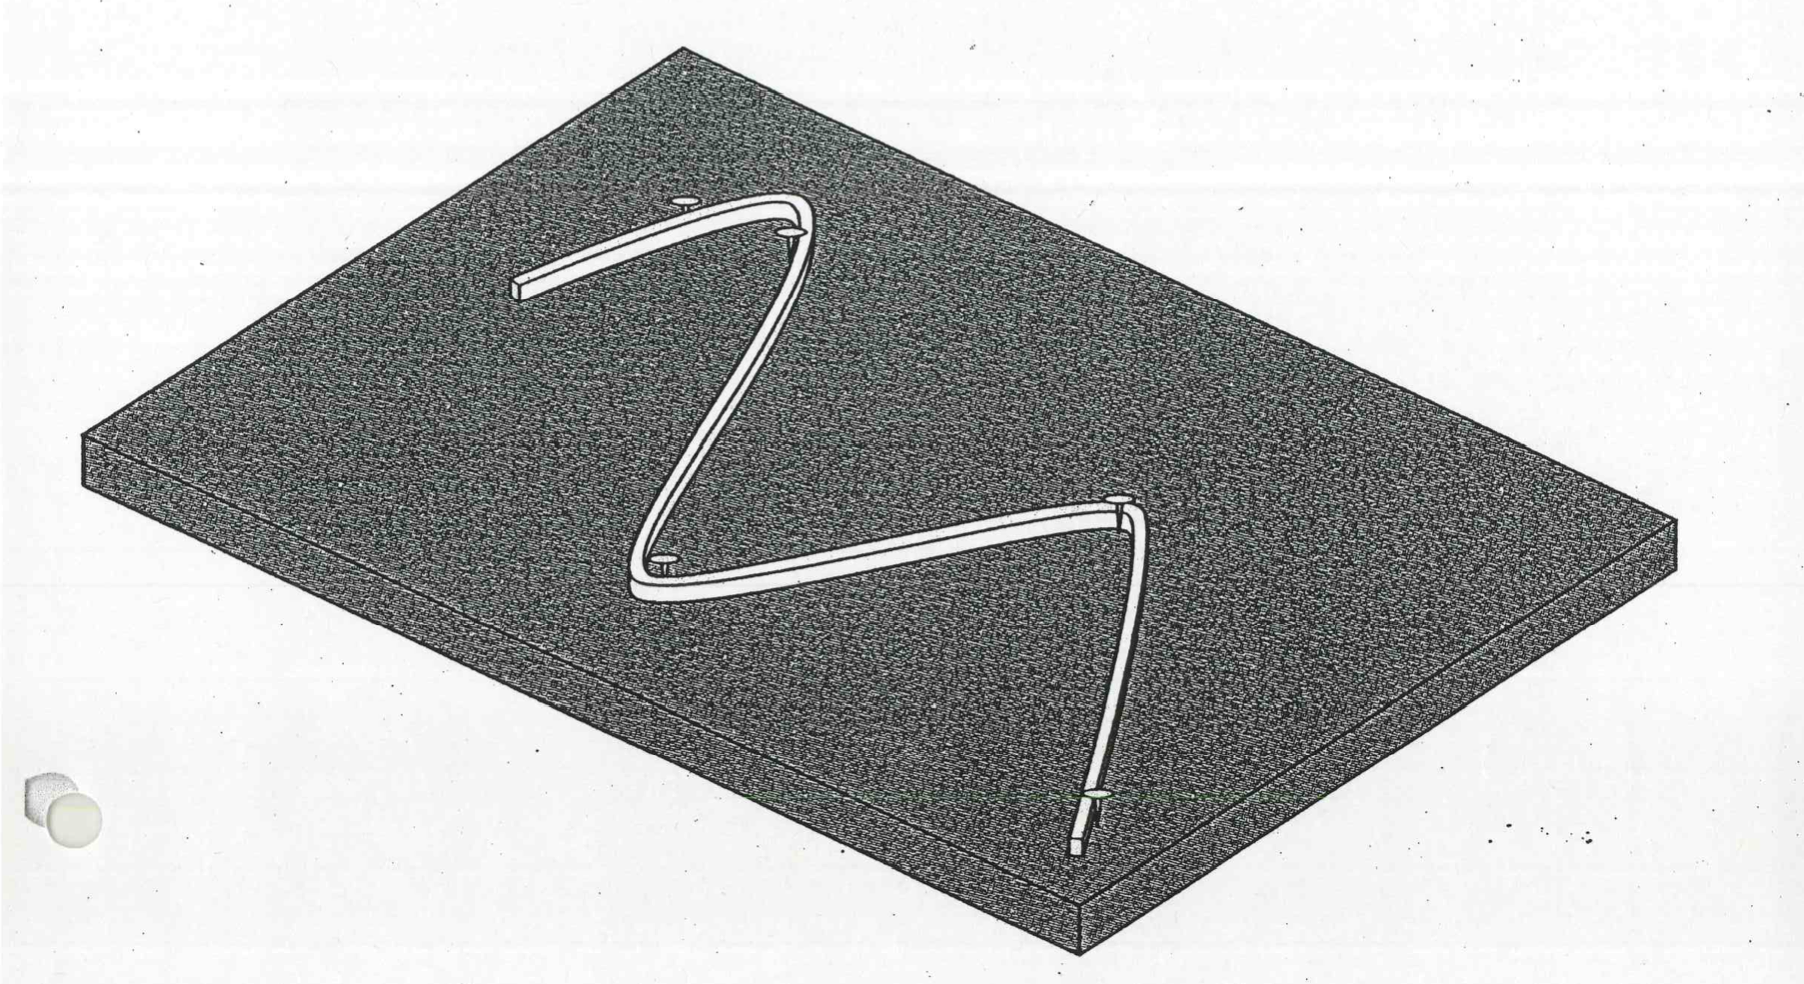
\includegraphics[scale=0.4]{physical_splines}
  \caption{Drafting technique of using a spline to draw smooth curves 
through a series of points}
  \label{fig:linear}
\end{figure}



Splines were first defined by Schoenberg in 1946. Note that the definition of a spline function does {\bf not} require that it interpolates some given function $f(x)$. But splines are often used as interpolating functions (a spline interpolant): 
\begin{itemize} 
\item They do not have the osciallatory nature of high degree interpolating polynomials 
\item the require no derivatives of $f(x)$, except possibly at the end points $x_0$ and $x_n$. 
\end{itemize} 

The most common spline interpolant is {\bf cubic}. 

\section{Cubic Spline Interpolants}


{\bf Definition:} Given $x_0,x_1,...,x_n$ with $x_i < x_{i+1}$ for each $i$, and $f(x_0), f(x_1), ..., f(x_n)$, then $S(x)$ is a {\bf cubic spline interpolant} for $f(x)$ if,

\begin{enumerate}[(a)]
\item{$S(x)$ is a cubic polynomial, denoted by $S_j(x)$, on each subinterval $[x_j,x_{j+1}]$, for $j=0,...,n-1$}
\item{$S_j(x_j)=f(x_j)$, for $j=0,...,n-1$ and $S_{n-1}(x_n)=f(x_n)$}
\item{$S_{j+1}(x_{j+1})=S_j(x_{j+1})$, for $j=0,...,n-2$}
\item{$S'_{j+1}(x_{j+1})=S'_j(x_{j+1})$, for $j=0,...,n-2$}
\item{$S''_{j+1}(x_{j+1})=S''_j(x_{j+1})$, for $j=0,...,n-2$}
\item{either one of the following hold:}
\begin{enumerate}[(i)]
\item{$S''(x_0)=S''(x_n)=0$ (natural bounds), or}
\item{$S'(x_0)=f'(x_0)$ and $S'(x_n)=f'(x_n)$ (clamped bounds)}
\end{enumerate}
\end{enumerate}


{\bf Notes:}
\begin{itemize}
\item{for any $f(x)$, there exist an infinite number of cubic splines satisfying conditions (a) - (e). Why?}
\item{There are $n$ cubic polynomials $S_j(x)$ to specify, each one is defined by 4 coefficients, giving a total of $4n$ unknowns to be specified.}
\item{However, condition (b) gives $n+1$ conditions to be satisfied, and (c), (d) and (e) each give $n-1$ conditions to be satisfied.}
\item{Thus, there are $(n+1)+3(n-1)=4n-2$ conditions (equations) to be satisfied in $4n$ unknowns.}
\item{But if either (i) or (ii) is also required to be satisfied, then there are $4n$ conditions in $4n$ unknowns and there exists a \underline{unique} cubic spline interpolant satisfying (a) - (f).}
\end{itemize}


\noindent
{\bf Example 1: Cubic Spline}

\noindent
Determine $a_0,b_0,d_0,a_1,b_1,c_1,$ and $d_1$ so that
\[
S(x) = \left\{
\begin{array}{ll}
     a_0+b_0x-3x^2+d_0x^3, & -1 \leq x\leq 0 \\
     a_1+b_1x+c_1x^2+d_1x^3, & 0 \leq x\leq 1 
\end{array}
\right. \]
is the natural cubic spline function such that $S(-1)=1, S(0)=2,S(1)=-1$.

\noindent
{\bf Solution}
Here, the cubic spline is expressed as
\[
S(x) = \begin{cases}
S_0(x)=a_0+b_0x-3x^2+d_0x^3, & \text{ if } 1 \leq x \leq 0 \\
S_1(x)=a_1+b_1x+c_1x^2+d_1x^3, & \text{ if } 0 \leq x \leq 1
\end{cases}
\]
and we have $x_0=-1,x_1=0,x_2=1,f(x_0)=1,f(x_1)=2,f(x_2)=-1$.

(b) \begin{equation}S_0(x_0)=f(x_0) \Rightarrow S_0(-1)=1 \Rightarrow a_0-b_0-3-d_0=1 \Rightarrow \boxed{a_0-b_0-d_0=4}\end{equation}.

\begin{equation}S_1(x_1)=f(x_1) \Rightarrow S_1(0)=2 \Rightarrow \boxed{a_1=2}\end{equation}.

\begin{equation}S_1(x_2)=f(x_2) \Rightarrow S_1(1)=-1 \Rightarrow a_1+b_1+c_1+d_1=-1 \Rightarrow \boxed{b_1+c_1+d_1=-3} \end{equation}.

(c) \begin{equation}S_1(x_1)=S_0(x_1) \Rightarrow S_1(0)=S_0(0) \Rightarrow a_1=a_0 \Rightarrow \boxed{a_0=2}\end{equation}.

(d) $S_0'(x) = b_0 -6x+3d_0x^2$ and $S_1'(x)=b_1+2c_1x+3d_1x^2$

thus

\begin{equation}S_1'(x_1)=S_0'(x_1) \Rightarrow S_1'(0)=S_0'(0) \Rightarrow b_1=b_0 \Rightarrow \boxed{b_1-b_0=0}\end{equation}.

(e)  $S_0''(x) = -6+6d_0x$ and $S_1''(x)=2c_1+6d_1x$

thus

\begin{equation}S_1''(x_1)=S_0''(x_1) \Rightarrow S_1''(0)=S_0''(0) \Rightarrow 2c_1=-6 \Rightarrow \boxed{c_1=-3}\end{equation}.

(f) To get the natural spline we use criteria (i):

\begin{equation}S_0''(x_0)=0 \Rightarrow S_0''(-1) = 0 \Rightarrow -6+6d_0(-1)=0 \Rightarrow \boxed{d_0=-1}\end{equation}.

\begin{equation}S_1''(x_2)=0 \Rightarrow S_1''(1)=0 \Rightarrow 2c_1+6d_1=0 \Rightarrow \boxed{d_1=1}\end{equation}.

So, we know that $a_0=2$, $a_1=1$, $c_1=-3$, $d_0=-1$ and $d_1=1$, that leaves the 2 unknowns $b_0$, and $b_1$ to solve. If we substitute $c_1$ and $d_1$ into equation (8) we get $b_1=-1$ and thus $b_0=-1$ by (10).

So finally the spline is,

\[
S(x) = \begin{cases}
2-x-3x^2-x^3, & \text{ if } -1 \leq x \leq 0 \\
2-x-3x^2+x^3, & \text{ if } 0 \leq x \leq 1
\end{cases}
\]

I plotted this spline in MATLAB with the following commands:

\begin{verbatim}
>> x=[-1,0,1];
>> y=[1,2,-1];
>> x0=[-1:0.1:0];
>> x1=[0:0.1:1];
>> S0=2-x0-3*x0.^2-x0.^3;
>> S1=2-x1-3*x1.^2+x1.^3;
>> plot(x,y,'*',x0,S0,x1,S1)
\end{verbatim}

\noindent
This results in the plot given in Figure 6.

\begin{figure} 
  \centering
  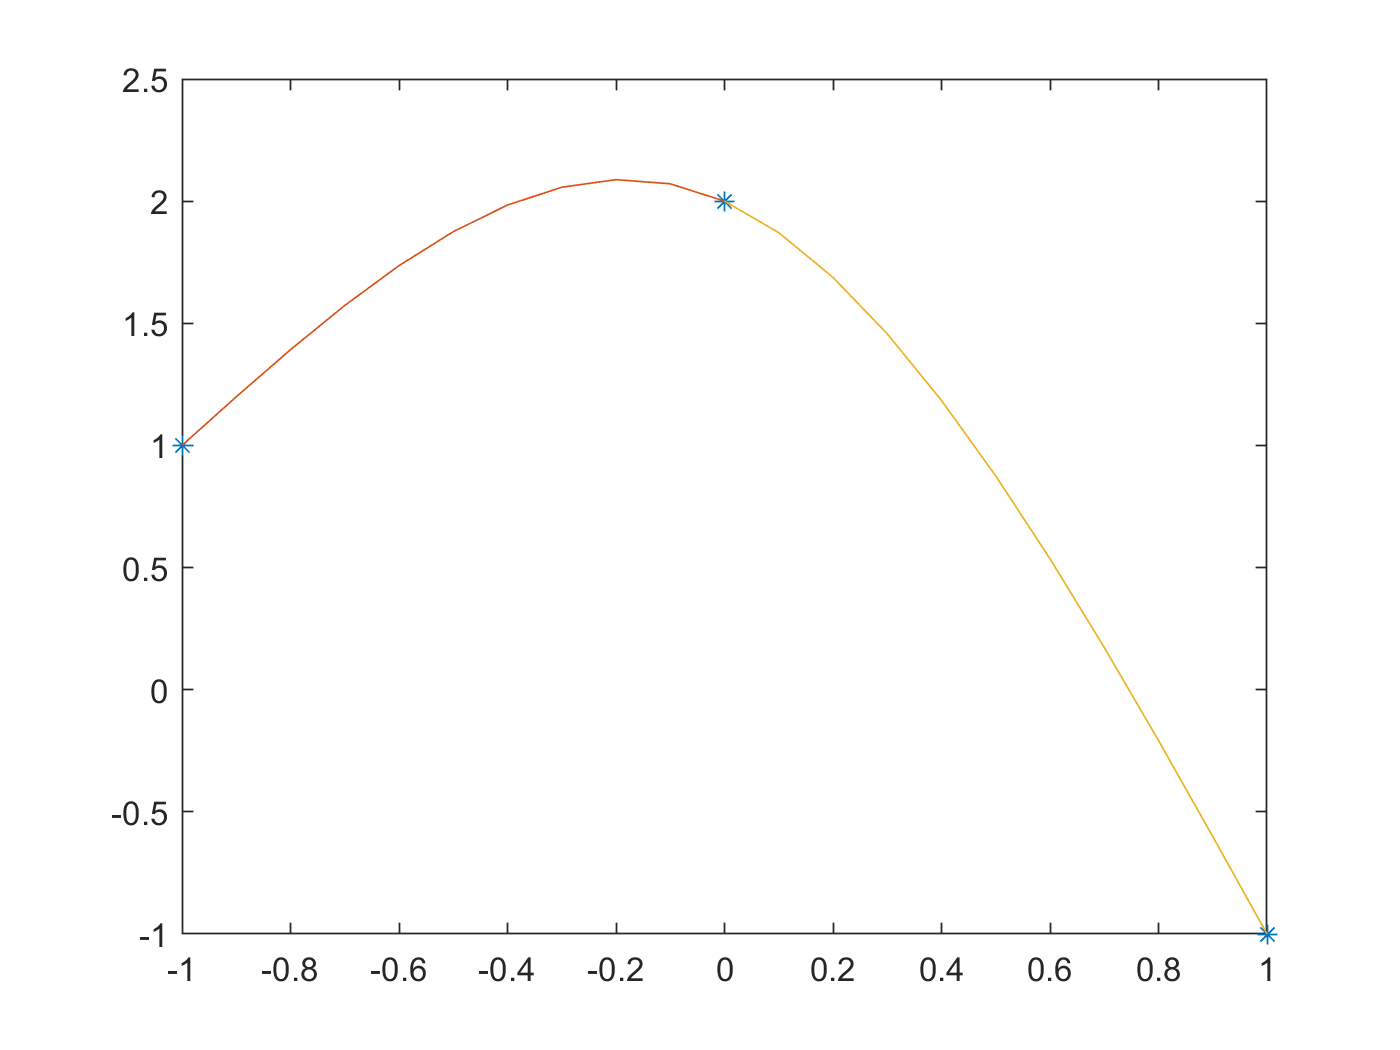
\includegraphics[scale=0.3]{lect14CubSpline}
  \caption{Cubic spline example}
  \label{fig:CubSpline}
\end{figure}

{\bf Cubic Splines in MATLAB}

There is an algorithm for spline computation given in the text but it has a different derivation than what we have done and different from MATLAB. In MATLAB they use a different form for the splines. For example, when $n=3$, MATLAB uses the following form for the cubic polynomials:
\begin{align*}
     S_0(x) &= a_0+b_0(x-x_0)+c_0(x-x_0)^2+d_0(x-x_0)^3 \\
     S_1(x) &= a_1+b_1(x-x_1)+c_1(x-x_1)^2+d_1(x-x_1)^3 \\
     S_2(x) &= a_2+b_2(x-x_2)+c_2(x-x_2)^2+d_2(x-x_2)^3
\end{align*}


Note that, with this form, $a_0=f(x_0), a_1=f(x_1),$ and $a_2=f(x_2)$. This simplifies the system somewhat. 

\section{Quadratic Spline Interpolants}
Construction of quadratic splines is similar to that of cubic splines but there are only $3n$ unknown coefficients and you do not need to set the second derivatives of the interior knots to be equal. That is, we do not create the (e) equations from above. As such, the (b) to (d) equations total $3n-1$, meaning that we also only need one extra (f) equation. Often we use $Q''(x_0)=0$ or, as is the case with the next example, we assign one of the coefficients before hand.

\noindent
{\bf Example 2: Quadratic Spline}

\noindent
Determine $a,b,c,d,$ and $e$ so that
\[
Q(x) = \left\{
\begin{array}{ll}
      ax^2+x+b, & -1 \leq x\leq 0 \\
     cx^2+dx+e, & 0 \leq x\leq 1 
\end{array}
\right. \]
is a quadratic spline function that interpolates $f(x)$ where $f(-1)=1, f(0)=1,f(1)=1$.


\noindent
{\bf Solution}

(a) Here, the quadratic spline is expressed as
\[
Q(x) = \begin{cases}
Q_0(x)=ax^2+x+b, & \text{ if } -1 \leq x \leq 0 \\
Q_1(x)=cx^2+dx+e, & \text{ if } 0 \leq x \leq 1
\end{cases}
\]
and we have $x_0=-1,x_1=0,x_2=1,f(x_0)=1,f(x_1)=1,f(x_2)=1$. Notice that I have given you one coefficient, meaning we only have five unkowns here and thus need only five equations. This means I won't need boundary conditions in this case (no (f) criteria). Also, for quadratic splines we never have the (e) conditions.

(b) \begin{equation}Q_0(x_0)=f(x_0) \Rightarrow Q_0(-1)=f(-1) \Rightarrow a-1+b=1 \Rightarrow \boxed{a+b=2} \end{equation}.

\begin{equation}Q_1(x_1)=f(x_1) \Rightarrow Q_1(0)=f(0) \Rightarrow \boxed{e=1}\end{equation}.

\begin{equation}Q_1(x_2)=f(x_2) \Rightarrow Q_1(1)=f(1) \Rightarrow \boxed{c+d+e=1}\end{equation}.

(c) \begin{equation}Q_1(x_1)=Q_0(x_1) \Rightarrow Q_1(0)=Q_0(0) \Rightarrow e=b \Rightarrow \boxed{e-b=0}\end{equation}.

(d) $Q_0'(x) = 2ax+1$ and $Q_1'(x)=2cx+d$

thus

\begin{equation}Q_1'(x_1)=Q_0'(x_1) \Rightarrow Q_1'(0)=Q_0'(0) \Rightarrow \boxed{d=1}\end{equation}.

Here, we need to solve the above system of five equations in five unknowns. This one is simple enough that we can do it manually with equation substitutions. Thus, substituting equations (2) and (5) in (3) we get $c=-1$. Substituting (2) in (4) gives $b=1$, and substituting that into (1) gives $a=1$.


So, $a=1, b=1, c=-1,d=1,e=1$ and so finally the spline is,

\[
Q(x) = \begin{cases}
x^2+x+1, & \text{ if } -1 \leq x \leq 0 \\
-x^2+x+1, & \text{ if } 0 \leq x \leq 1
\end{cases}
\]

I plotted this spline in MATLAB with the following commands:

\begin{verbatim}
>> x=[-1,0,1]

x =

    -1     0     1

>> y=[1,1,1]

y =

     1     1     1

>> plot(x,y,'*')
>> hold on
>> x0=[-1:0.1:0];
>> q0=x0.^2+x0+1;
>> x1=[0:0.1:1];
>> q1=-x1.^2+x1+1;
>> plot(x0,q0,x1,q1)
\end{verbatim}

\noindent
This results in the plot given in Figure 5.

\begin{figure} 
  \centering
  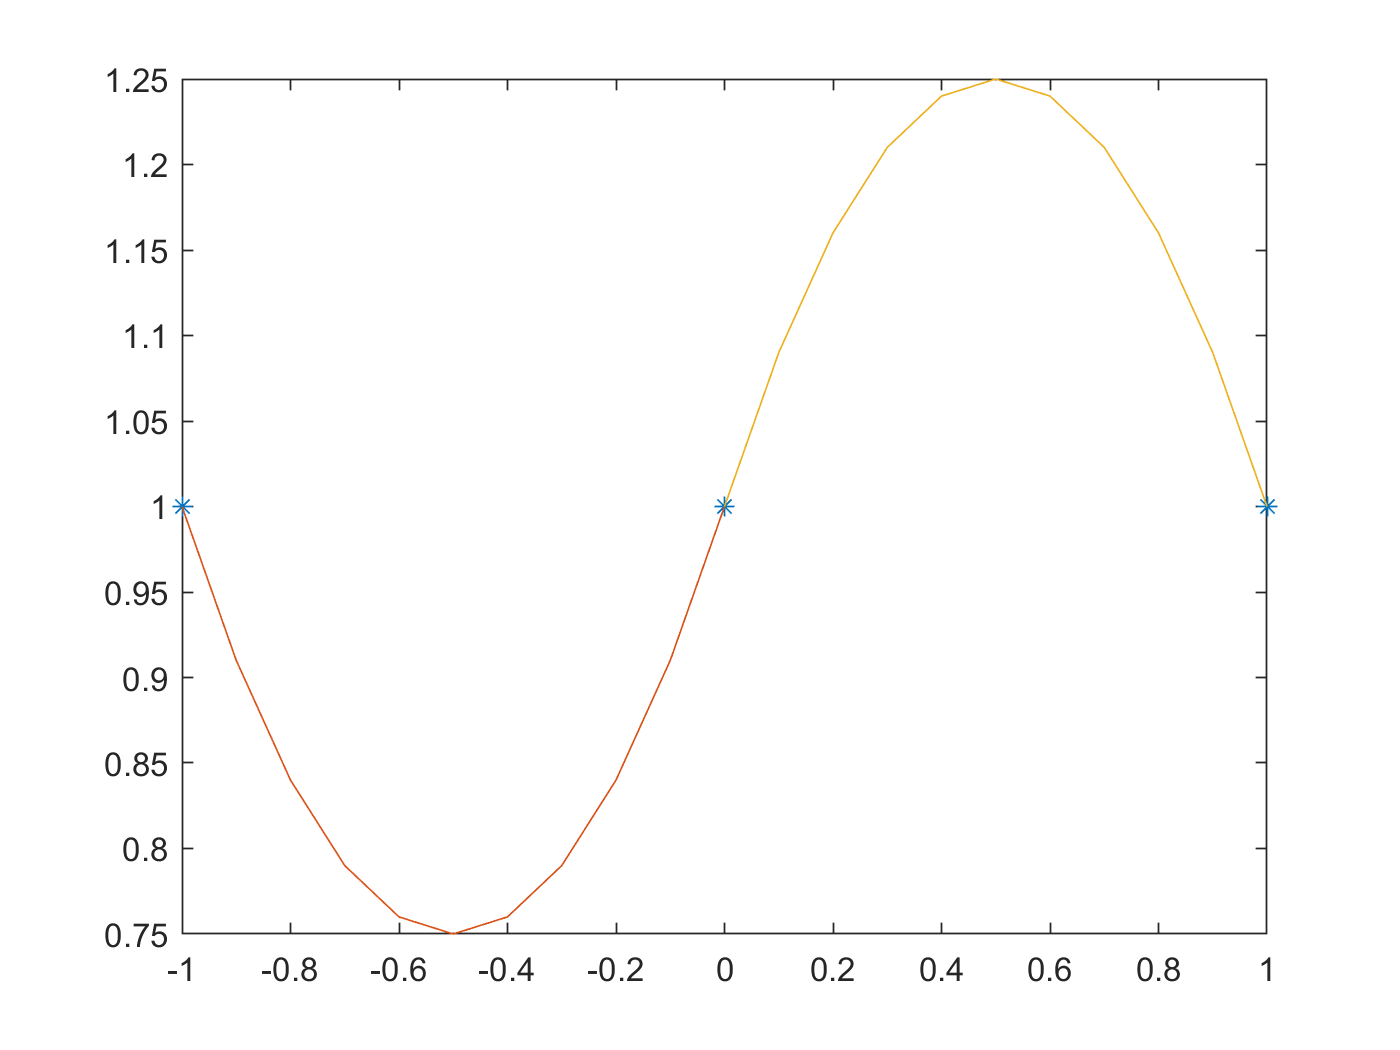
\includegraphics[scale=0.3]{lect14QuadSpline}
  \caption{Quadratic spline example}
  \label{fig:QuadSpline}
\end{figure}


\end{document} 















